\documentclass{article}
\usepackage{amsthm}
\usepackage{amsmath}
\usepackage{etoc}
\usepackage{amssymb}
\usepackage{enumitem}
\usepackage{apacite}
\usepackage{mathtools, amssymb}
\usepackage{bm}
\usepackage{tikz}
\usepackage{fancyhdr}
\usepackage{caption}
\usepackage{tabto}
\usepackage{hyperref}
\usepackage{graphicx}
\usepackage[nottoc]{tocbibind}
\usepackage{calrsfs}
\usepackage{changepage}
\usepackage{siunitx}
\usepackage{listings}% http://ctan.org/pkg/listings
\lstset{
  basicstyle=\ttfamily,
  mathescape
}
\usetikzlibrary{arrows.meta, automata, positioning, quotes}



% Margins
\usepackage[top=2.5cm, left=3cm, right=3cm, bottom=4.0cm]{geometry}
% Colour table cells

% Get larger line spacing in table
\newcommand{\tablespace}{\\[1.25mm]}
\newcommand\Tstrut{\rule{0pt}{2.6ex}}         % = `top' strut
\newcommand\tstrut{\rule{0pt}{2.0ex}}         % = `top' strut
\newcommand\Bstrut{\rule[-0.9ex]{0pt}{0pt}}   % = `bottom' strut

%%%%%%%%%%%%%%%%%
%     Title     %
%%%%%%%%%%%%%%%%%
\title{Theory of automata and Formal languages}
\author{Fernando Javier López Cerezo \\ Practice 4}
\date{\today}

\begin{document}
\maketitle

\section*{Problem 1}
Exercise 1 asks us to find a while program that diverges with the smallest possible codification. This is my contribution: \begin{lstlisting}
Diverge=(0,s)
s:
   while X1 $\neq$  1 do
      X1 := 0;
   od
\end{lstlisting}
This program has the following codification: \\\\ 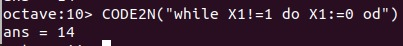
\includegraphics[width=\linewidth]{diverge.png}


\section*{Problem 2}
Problem 2 asks us to code in octave a program which prints all vectors belonging to $\mathbb{N}^*$. As there are infinite vectors I tried doing a program with an infinite loop that would print in screen all the vectors one by one, this program would of course be neverending. However I don't think octave allows this as when I tried no output was shown on-screen until I interrupted the program. So instead I created a program that outputs the first n vectors. 
\begin{lstlisting}
for i=0:n-1
	disp([num2str(i+1), ': (' num2str(godeldecoding(i)) ')']);
	i=i+1;
	end
end
\end{lstlisting} 
Here is an example of it's execution: \\\\ 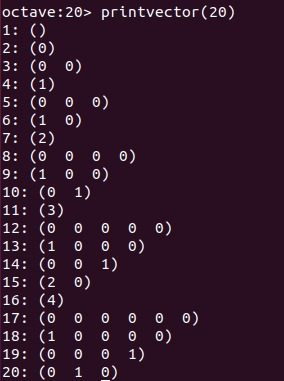
\includegraphics[width=\linewidth]{printvector.png}

\section*{Problem 3}
Problem 3 asks us to do the same as problem 2 but in this case the output should be all possible while programs instead of vectors. Therefore:
\begin{lstlisting}
for i=0:n-1
	disp([num2str(i+1), ': (' num2str(N2WHILE(i)) ')']);
	i=i+1;
	end
end
\end{lstlisting} 
Here is an example of it's execution: \\\\ 
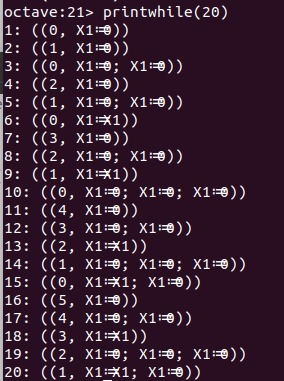
\includegraphics[width=\linewidth]{printwhile.png}

\end{document}